\documentclass[12pt]{article}

\usepackage[margin=1in]{geometry}
\usepackage{amsmath,amsthm,amssymb}
\usepackage{fancyhdr}
\usepackage[small,compact]{titlesec}
\usepackage{float}

\lhead{Erich Menge}
\chead{\classnameandsection}
\rhead{\homeworktitle}

\pagestyle{fancy}

\newcommand{\sethomeworknumber}[1]{
  \newcommand{\homeworktitle}{Homework #1}
}

\newcommand{\N}{\mathbb{N}}
\newcommand{\Z}{\mathbb{Z}}
\newcommand{\homeworkheader}[1]{
  \title{\vspace{2in}\homeworktitle}
  \author{Erich Menge (X.500: menge053, Student ID: 4624713) \\
  #1}
  \maketitle
  \newpage
}

\newenvironment{problem}[1]{
  \ignorespaces
  \section*{Problem #1}
}{
  \ignorespacesafterend
}

\newenvironment{solution}{
  \ignorespaces
  \subsection*{Solution}
}{
  \ignorespacesafterend
}

\newcommand{\classnameandsection}{CSCI 4011 Formal Languages And Automata Theory Section 3}


\sethomeworknumber{9}

\begin{document}
\homeworkheader{\classnameandsection}

\begin{problem}{23.1-3}
  Show that if an edge $(u,v)$ is contained in some minimum spanning tree, then it is a light edge crossing some cut of
  the graph.
  \begin{solution}
    By definition a light edge crossing the cut is a minimum weight edge. When we have some graph $G$ we can expand a
    minimum spaning tree such that each edge of the spanning tree is the minimum weight edge, or equal to some minimum
    weight edge of G.

    Since each edge of the minimum spanning tree maintains this invariant where $A$ is a subset of edges of the minimum
    spanning tree we know that the edge $(u,v)$ exists in that set $A$ which maintains the invariant. That means that
    there must exist some cut in which edge $(u,v)$ is a light edge. If it wasn't, the invariant wouldn't hold for that
    edge (there would be some other edge that would be a lighter weight, violating the definition of a minimum spanning
    tree).  Thus $(u,v)$ must be a light edge in some cut of the graph.
  \end{solution}
\end{problem}

\begin{problem}{23.1-7}
  Argue that if all edge weights of a graph are positive, then any subset of edges that connects all vertices and has
  minimum total weight must be a tree. Give an example to show that the same conclusion does not follow if we allow some
  weights to be nonpositive.
  \begin{solution}
    In the case that all edge weights are positive we know that if we have some set of edges connecting all verticies
    and the weight is a minimum weight it must be a minimum weight spanning tree because if we were to replace any any
    of the edges in the tree with an edge of higher weight we could no longer have a minimum weight tree, since by
    definition in the problem the tree must have minimum weight.

    In the case of a mixture of negative and positive weights we cannot be sure that we don't have some cycle that was
    chosen with a negative value, creating a sum of edges that give a minimum weight but contain an additional edge that
    is not allowed.
    \begin{figure}[H]
      \centering
      \caption{Potential Sub-Graphs}
      \subfigure[No Negatives]{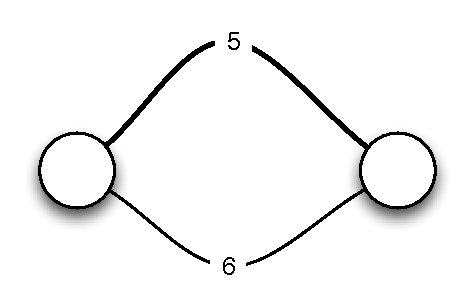
\includegraphics{23_1_7_a.eps}}
      \subfigure[Negatives Allowed]{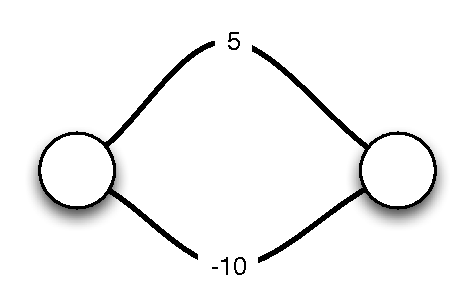
\includegraphics{23_1_7_b.eps}}
    \end{figure}
  \end{solution}
\end{problem}

\begin{problem}{23.1-8}
  Let T be a minimum spanning tree of a graph G, and let L be the sorted list of the edge weights of T. Show that for
  any other minimum spanning tree $T'$ of G, the list L is also the sorted list of edge weights of $T'$.
  \begin{solution}
    For each iteration of the spanning tree algorithm the invariant must be maintained. That is the greedy choice that
    the edge selected is a minimum weight edge.  More than one minimum weight edge may exist, but that means the weights
    are equal, so no matter how you select the edge the weight entered on the list $L$ will be the same. This continues
    for the next edge and so on.

    If one list of edge weights differed than another it would mean that some edge was a higher weight than another
    particular edge which would mean that the greedy choice was not selected for some edge. Thus the list with the
    greater weight edge was not an optimal solution and the tree must not be a minimum spanning tree.

    So for any particular graph $G$ there may be many different spanning trees, but because these differences result in
    being able to choose more than one edge with the same weight, the sorted list of weights must be the same.
  \end{solution}
\end{problem}

\begin{problem}{23.1-9}
  Let T be a minimum spanning tree of a graph $G = (V,E)$, and let $V'$ be a subset of $V$. Let $T'$ be the subgraph of
  $T$ induced by $V'$, and let $G'$ be the subgraph of $G$ induced by $V'$. Show that if $T'$ is connected, then $T'$ is
  a minimum spanning tree of $G'$.
  \begin{solution}
    Because $T'$ is a sub graph of $T$ and $T$ is a minimum spanning tree if we were to assume that $T'$ is not a
    minimum spanning tree that would mean that there is some edge in $T'$ that is not a minimum weight edge so that the
    invariant doesn't hold. This means we could replace this edge with the lighter weight edge but if we can do this it
    must mean we do not have a minimum spanning tree so it is a contradiction. Thus if $T'$ is a subgraph of $T$ and $T$
    is a minimum spanning tree $T'$ must also be a minimum spanning tree. Because if it wasn't, it could be improved,
    but if it could be improved then $T$ could have a lower total weight meaning it must not be a MST.
  \end{solution}
\end{problem}

\begin{problem}{23.2-1}
  Kruskal's algorithm can return different spanning trees for the same input graph G, depending on how it breaks ties
  when the edges are sorted into order. Show that for each minimum spanning tree $T$ of $G$, there is a way to sort the
  edges of $G$ in Kruskal's algorithm so that the algorithm returns $T$.
  \begin{solution}
    The reason Kruskal's algortithm may return different spanning trees is the given algorithm simply orders by weight.
    In the event that two edges have the same minimum weight the alrogirthm in the book does not specify the selection
    of that particular minimum weight edge.  So depending on specific algorithm implementation two correct
    implementations could return different spanning trees.

    If we were to add an aditional rule to the algorithm that we sort by minimum weight edge and by the vertex order
    (i.e. always select the minimum weight edge to the vertex that appears in the list of vertices first) we can ensure
    that for every graph $G$ there is only one MST $T$.
  \end{solution}
\end{problem}

\begin{problem}{23.2-2}
  Suppose that we represent the graph $G = (V,E)$ as an adjacency matrix. Give a simple implementation of Prim's
  algorithm for this case that runs in $O(V^2)$ time.
  \begin{solution}
    We can use a modified version of the algorithm in the book. Since in an adjacency matrix we have $|V|$ rows and $|V|$
    columns it is a $|V| \times |V|$ matrix. The main loop iterates over all the verticies, so that is $O(V)$. Then we need
    to check the corresponding row in the adjacency matrix, which has $|V|$ columns. This matrix check is done in each of
    the main loops, so it is done $V$ times. So we have $O(V^2)$. Note that only the row needs to be checked because it
    is not directed, and thus the adjacency matrix is symmetric so there is no need to check the corresponding column as
    well.
    \begin{lstlisting}[mathescape]
      MST-Prim(G, w, r)
        for each $u \in$ G.V
          u.key = $\infty$
          u.$\pi$ = NIL
        r.key = 0
        Q = G.V
        while Q $\ne$ $\emptyset$
          u = Extract-Min(Q)
          for each v $\in$ G.AdjMatrix[G.rowof(u)][0..|V| - 1]
            if v $\in$ Q and w(u,v) < v.key
              v.$\pi$ = u
              v.key = w(u,v)
    \end{lstlisting}
  \end{solution}
\end{problem}

\end{document}
